\appendix
\section{Compute Costs}
Experiments were collected using a mix of a local RTX 3090 and AWS-hosted Tesla T4 GPUs.
The total cost of cloud compute was approximately \textbf{\$130}.
Over \textbf{312} training runs were logged in Weights \& Biases, totaling approximately \textbf{566.59 GPU hours}.
The estimated carbon footprint of the compute used is approximately \textbf{A kg CO$_2$e}, based on the methodology from \citet{lacoste-2019-carbontracker}.

\section{AI Usage}

This paper utilized artificial intelligence tools in the following ways:
\begin{itemize}
    \item \textbf{GitHub Copilot (Claude Sonnet 4.5)} was used for typesetting assistance with LaTeX/KaTeX, IDE autocomplete suggestions during coding, and to occassionally perform straightforward refactorings, CUDA performance optimizations, and debugging.
    \item \textbf{ChatGPT (GPT-5.1)} was used for brainstorming ideas for reinforcement learning applications in games, guidance in hyperparameter tuning, helping to outline the structure of this paper, assistance in discovering relevant research and citations, and for writing tone and quality feedback.
\end{itemize}
All other content, including research methodology, analysis, results interpretation, and conclusions, represents original work by the author. The AI tools were not used to generate substantive content or analysis in this document.


\section{Hyperparameters}
The following hyperparameters were used for the baseline models:

\begin{table}[!htbp]
    \centering
    \small
    \caption{Shared hyperparameters across all algorithms}
    \label{tab:shared-hyperparameters}
    \begin{tabular}{lc}
        \hline
        \textbf{Hyperparameter}       & \textbf{Value} \\
        \hline
        $d_h$ (Hidden Size)           & 600            \\
        $L$ (Hidden Layers)           & 3              \\
        $p_d$ (Dropout Rate)          & 0.1            \\
        $r_{\alpha}$ (Min LR Ratio)   & 0.01           \\
        $B$ (Games per Batch)         & 20             \\
        Activation Function           & Swish          \\
        Rolling Action Representation & Categorical    \\
        \hline
    \end{tabular}
\end{table}

\begin{table}[!htbp]
    \centering
    \small
    \setlength{\tabcolsep}{4pt}
    \caption{Algorithm-specific hyperparameters}
    \label{tab:algorithm-hyperparameters}
    \begin{tabular}{lccc}
        \hline
        \textbf{Hyperparameter}        & \textbf{REINFORCE} & \textbf{A2C} & \textbf{PPO} \\
        \hline
        $\alpha$                       & 0.001              & 0.0001       & 0.0001       \\
        $\gamma$ (min)                 & 0.95               & 0.99         & 0.99         \\
        $\gamma$ (max)                 & 1.0                & 0.99         & 0.99         \\
        $\tau_{\mathrm{clip}}$         & 0.0                & 1.0          & 1.0          \\
        $\lambda_V$                    & 0.025              & 0.005        & 0.01         \\
        $\beta_{\mathrm{roll}}$ (max)  & 0.1                & 0.06         & 0.02         \\
        $\beta_{\mathrm{roll}}$ (min)  & 0.01               & 0.02         & 0.005        \\
        $\beta_{\mathrm{score}}$ (max) & 0.02               & 0.03         & 0.05         \\
        $\beta_{\mathrm{score}}$ (min) & 0.003              & 0.008        & 0.01         \\
        Entropy Hold Period            & 0.1                & 0.3          & 0.1          \\
        Entropy Anneal Period          & 0.55               & 0.6          & 0.8          \\
        \hline
    \end{tabular}
\end{table}

\begin{table}[!htbp]
    \centering
    \small
    \caption{PPO-specific hyperparameters}
    \label{tab:ppo-hyperparameters}
    \begin{tabular}{lc}
        \hline
        \textbf{Hyperparameter} & \textbf{Value} \\
        \hline
        PPO Clip $\epsilon$     & 0.2            \\
        PPO Games per Minibatch & 4              \\
        PPO Epochs              & 3              \\
        \hline
    \end{tabular}
\end{table}

\section{Yahtzee Scoring Rules}
\label{app:scoring}
Next we define the indicator functions for each of the scoring categories:

\begin{align*}
    \mathbb{I}_{3\mathrm{k}}(\mathbf{d})
     & = \mathbb{I}\bigl\{ \max_{v} n_v(\mathbf{d}) \ge 3 \bigr\} \\
    \mathbb{I}_{4\mathrm{k}}(\mathbf{d})
     & = \mathbb{I}\bigl\{ \max_{v} n_v(\mathbf{d}) \ge 4 \bigr\} \\
    \mathbb{I}_{\mathrm{full}}(\mathbf{d})
     & = \mathbb{I}\Bigl\{
    \exists i, j \in \{1, \mathellipsis, 6 \} \ \text{with} \ n_i(\mathbf{d}) = 3 \land n_j(\mathbf{d}) = 2
    \Bigr\}                                                       \\
    \mathbb{I}_{\mathrm{ss}}(\mathbf{d})
     & = \mathbb{I}\Bigl\{
    \exists k \in \{1,2,3\} \ \text{with}\
    \sum_{v=k}^{k+3} \mathbb{I}\{n_v(\mathbf{d}) > 0\} = 4
    \Bigr\}                                                       \\
    \mathbb{I}_{\mathrm{ls}}(\mathbf{d})
     & = \mathbb{I}\Bigl\{
    \exists k \in \{1,2\} \ \text{with}\
    \sum_{v=k}^{k+4} \mathbb{I}\{n_v(\mathbf{d}) > 0\} = 5
    \Bigr\}                                                       \\
    \mathbb{I}_{\mathrm{yahtzee}}(\mathbf{d})
     & = \mathbb{I}\bigl\{\max_v n_v(\mathbf{d}) = 5\bigr\}
\end{align*}

The potential score for each category can then be defined as:
\begin{align*}
    f_j(\mathbf{d})        & = j \cdot n_j(\mathbf{d}), \qquad j \in \{1,\dots,6\}                   \\
    f_7(\mathbf{d})        & = \mathbf{1}^\top \mathbf{d} \cdot \mathbb{I}_{3\mathrm{k}}(\mathbf{d}) \\
    f_8(\mathbf{d})        & = \mathbf{1}^\top \mathbf{d} \cdot \mathbb{I}_{4\mathrm{k}}(\mathbf{d}) \\
    f_9(\mathbf{d})        & = 25 \cdot \mathbb{I}_{\mathrm{full}}(\mathbf{d})                       \\
    f_{10}(\mathbf{d})     & = 30 \cdot \mathbb{I}_{\mathrm{ss}}(\mathbf{d})                         \\
    f_{11}(\mathbf{d})     & = 40 \cdot \mathbb{I}_{\mathrm{ls}}(\mathbf{d})                         \\
    f_{12}(\mathbf{d})     & = 50 \cdot \mathbb{I}_{\mathrm{yahtzee}}(\mathbf{d})                    \\
    f_{13}(\mathbf{d})     & = \mathbf{1}^\top \cdot \mathbf{d}                                      \\
    \mathbf{f}(\mathbf{d}) & =
    \bigl(f_1(\mathbf{d}), f_2(\mathbf{d}), \ldots, f_{13}(\mathbf{d})\bigr)
\end{align*}

\section{State Transition Function}
\label{app:transition-function}

$P$ can be defined by the following generative process.

\begin{itemize}
    \item If $r < 2$ and $a = k$, for each die $i$:
          \begin{itemize}
              \item if $k_i = 1$, keep $d'_i = d_i$;
              \item else sample $d'_i \sim \mathrm{Unif}\{1,\dots,6\}$ independently.
          \end{itemize}
          Set $c' = c,\ r' = r+1,\ t' = t$.
    \item If $r = 2$ and $a = i$, set $d' = d$, update $c' = \mathrm{score}(c,d,i)$,
          set $r' = 0,\ t' = t+1$.
\end{itemize}


\begin{table}[!htbp]
    \centering
    \small
    \caption{Category statistics (placeholder data)}
    \label{tab:category-stats}
    \begin{tabular}{lcc}
        \hline
        \multicolumn{1}{c}{\emph{Category}} & $\bar{s}(c)$ & $\sigma^{2}(c)$ \\
        \hline
        Ones                                & $<X>$        & $<Y>$           \\
        Twos                                & $<X>$        & $<Y>$           \\
        Threes                              & $<X>$        & $<Y>$           \\
        Fours                               & $<X>$        & $<Y>$           \\
        Fives                               & $<X>$        & $<Y>$           \\
        Sixes                               & $<X>$        & $<Y>$           \\
        Three of a Kind                     & $<X>$        & $<Y>$           \\
        Four of a Kind                      & $<X>$        & $<Y>$           \\
        Full House                          & $<X>$        & $<Y>$           \\
        Small Straight                      & $<X>$        & $<Y>$           \\
        Large Straight                      & $<X>$        & $<Y>$           \\
        Chance                              & $<X>$        & $<Y>$           \\
        Yahtzee                             & $<X>$        & $<Y>$           \\
        Upper Bonus                         & $<X>$        & $<Y>$           \\
        Yahtzee Bonus                       & $<X>$        & $<Y>$           \\
        \hline
    \end{tabular}
\end{table}



\begin{figure}[!htbp]
    \centering
    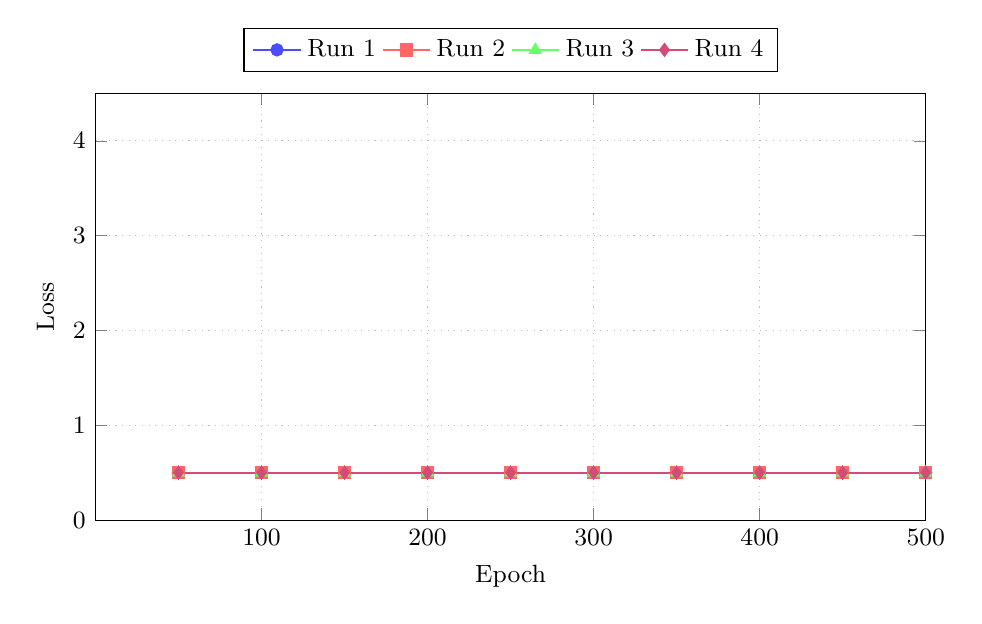
\begin{tikzpicture}
        \begin{axis}[
                width=\columnwidth,
                height=7cm,
                xlabel={Epoch},
                ylabel={Loss},
                xmin=0, xmax=500,
                ymin=0, ymax=4.5,
                xtick={100,200,300,400,500},
                grid=both,
                grid style={dotted},
                tick label style={font=\small},
                label style={font=\small},
                legend style={at={(0.5,1.05)},anchor=south,legend columns=4,font=\small},
                mark options={solid},
            ]

            % --- Run 1 (placeholder data around 1) ---
            \addplot[blue!70!white, thick, mark=*] coordinates {
                    ( 50,0.5) (100,0.5) (150,0.5) (200,0.5) (250,0.5)
                    (300,0.5) (350,0.5) (400,0.5) (450,0.5) (500,0.5)
                };

            % --- Run 2 (placeholder data around 2) ---
            \addplot[red!60!white, thick, mark=square*] coordinates {
                    ( 50,0.5) (100,0.5) (150,0.5) (200,0.5) (250,0.5)
                    (300,0.5) (350,0.5) (400,0.5) (450,0.5) (500,0.5)
                };

            % --- Run 3 (placeholder data around 3) ---
            \addplot[green!60!white, thick, mark=triangle*] coordinates {
                    ( 50,0.5) (100,0.5) (150,0.5) (200,0.5) (250,0.5)
                    (300,0.5) (350,0.5) (400,0.5) (450,0.5) (500,0.5)
                };

            % --- Run 4 (placeholder data around 4) ---
            \addplot[purple!70!white, thick, mark=diamond*] coordinates {
                    ( 50,0.5) (100,0.5) (150,0.5) (200,0.5) (250,0.5)
                    (300,0.5) (350,0.5) (400,0.5) (450,0.5) (500,0.5)
                };

            \legend{Run 1,Run 2,Run 3,Run 4}

        \end{axis}
    \end{tikzpicture}
    \caption{Training loss (placeholder data)}
    \label{fig:loss-vs-epoch}
\end{figure}
